\documentclass{standalone}
\usepackage{tikz}
\usetikzlibrary{patterns, positioning}


\begin{document}
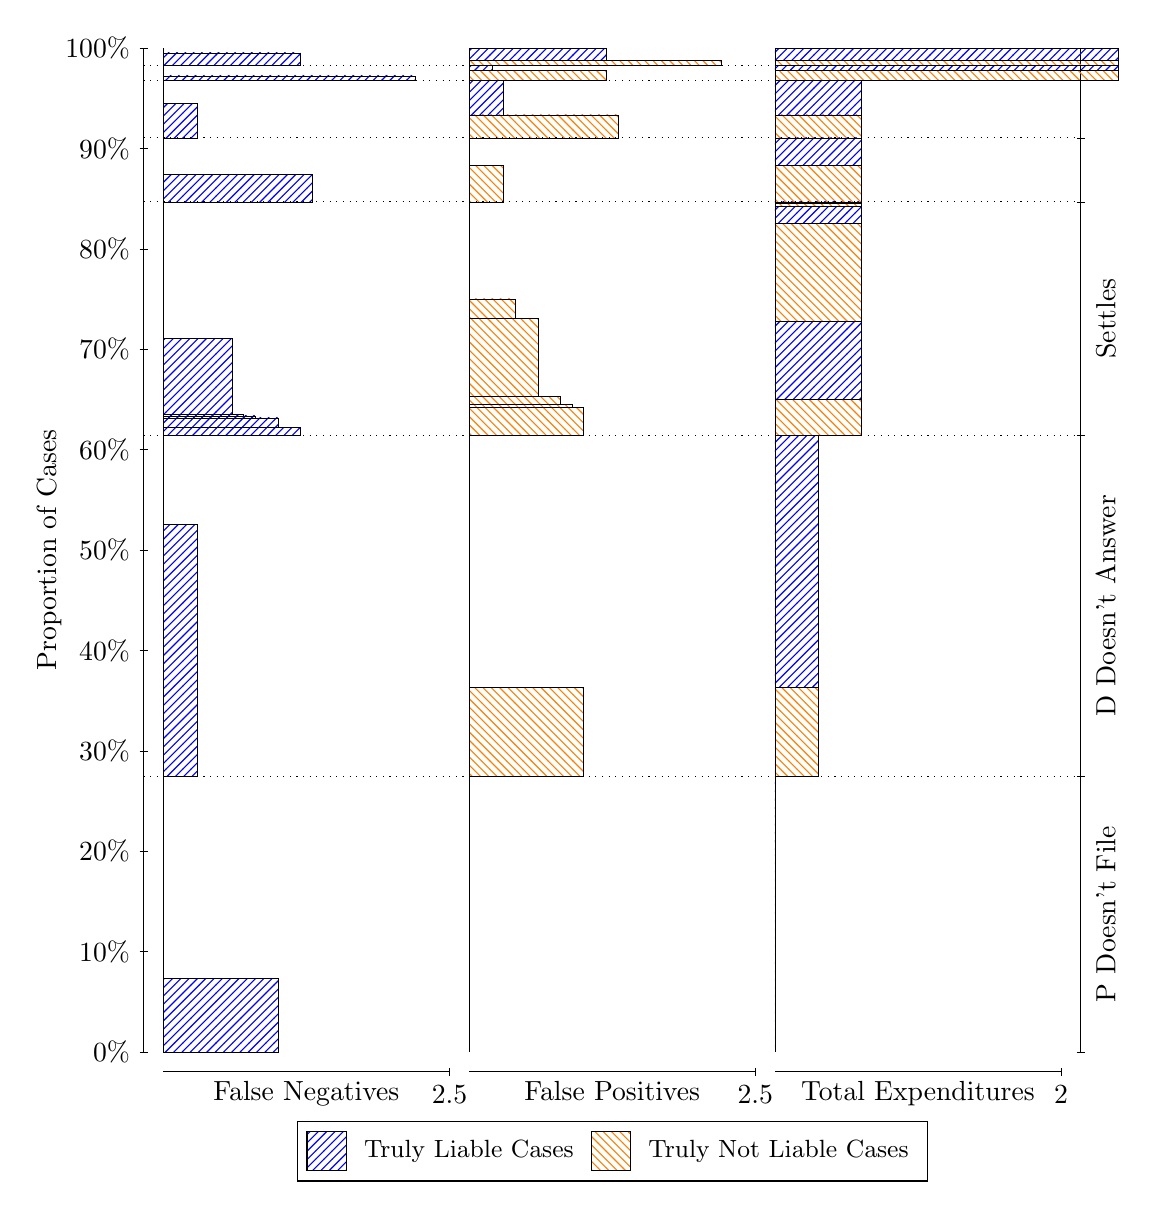
\begin{tikzpicture}
\draw[black, very thin] (1.5,1.75) -- (1.5,14.5);
\node[rotate=90, text=black, anchor=center] at (0.3, 8.125) {Proportion of Cases};
\draw[black, very thin] (1.45,1.75) -- (1.55,1.75);
\node[text=black, anchor=east] at (1.45, 1.75) {0\%};
\draw[black, very thin] (1.45,3.025) -- (1.55,3.025);
\node[text=black, anchor=east] at (1.45, 3.025) {10\%};
\draw[black, very thin] (1.45,4.3) -- (1.55,4.3);
\node[text=black, anchor=east] at (1.45, 4.3) {20\%};
\draw[black, very thin] (1.45,5.575) -- (1.55,5.575);
\node[text=black, anchor=east] at (1.45, 5.575) {30\%};
\draw[black, very thin] (1.45,6.85) -- (1.55,6.85);
\node[text=black, anchor=east] at (1.45, 6.85) {40\%};
\draw[black, very thin] (1.45,8.125) -- (1.55,8.125);
\node[text=black, anchor=east] at (1.45, 8.125) {50\%};
\draw[black, very thin] (1.45,9.4) -- (1.55,9.4);
\node[text=black, anchor=east] at (1.45, 9.4) {60\%};
\draw[black, very thin] (1.45,10.675) -- (1.55,10.675);
\node[text=black, anchor=east] at (1.45, 10.675) {70\%};
\draw[black, very thin] (1.45,11.95) -- (1.55,11.95);
\node[text=black, anchor=east] at (1.45, 11.95) {80\%};
\draw[black, very thin] (1.45,13.225) -- (1.55,13.225);
\node[text=black, anchor=east] at (1.45, 13.225) {90\%};
\draw[black, very thin] (1.45,14.5) -- (1.55,14.5);
\node[text=black, anchor=east] at (1.45, 14.5) {100\%};

\draw[black, very thin] (13.4,1.75) -- (13.4,14.5);
\draw[black, very thin] (13.35,1.75) -- (13.45,1.75);
\node[anchor=west] at (13.35, 1.75) {};
\draw[black, very thin] (13.35,5.2507) -- (13.45,5.2507);
\node[anchor=west] at (13.35, 5.2507) {};
\draw[black, very thin] (13.35,9.5821) -- (13.45,9.5821);
\node[anchor=west] at (13.35, 9.5821) {};
\draw[black, very thin] (13.35,12.547) -- (13.45,12.547);
\node[anchor=west] at (13.35, 12.547) {};
\draw[black, very thin] (13.35,13.359) -- (13.45,13.359);
\node[anchor=west] at (13.35, 13.359) {};
\draw[black, very thin] (13.35,14.085) -- (13.45,14.085);
\node[anchor=west] at (13.35, 14.085) {};
\draw[black, very thin] (13.35,14.282) -- (13.45,14.282);
\node[anchor=west] at (13.35, 14.282) {};
\draw[black, very thin] (13.35,14.5) -- (13.45,14.5);
\node[anchor=west] at (13.35, 14.5) {};

\draw[black, very thin, pattern color=blue, pattern=north east lines] (1.75,1.75) rectangle (3.2033,2.6881);
\draw[black, very thin, pattern color=orange, pattern=north west lines] (1.75,2.6881) rectangle (1.75,5.2507);
\draw[black, very thin, pattern color=blue, pattern=north east lines] (1.75,5.2507) rectangle (2.186,8.4549);
\draw[black, very thin, pattern color=orange, pattern=north west lines] (1.75,8.4549) rectangle (1.75,9.5821);
\draw[black, very thin, pattern color=blue, pattern=north east lines] (1.75,9.5821) rectangle (3.494,9.6777);
\draw[black, very thin, pattern color=blue, pattern=north east lines] (1.75,9.6777) rectangle (3.2033,9.8029);
\draw[black, very thin, pattern color=blue, pattern=north east lines] (1.75,9.8029) rectangle (2.9127,9.827);
\draw[black, very thin, pattern color=blue, pattern=north east lines] (1.75,9.827) rectangle (2.7673,9.8473);
\draw[black, very thin, pattern color=blue, pattern=north east lines] (1.75,9.8473) rectangle (2.622,10.815);
\draw[black, very thin, pattern color=orange, pattern=north west lines] (1.75,10.815) rectangle (1.75,12.547);
\draw[black, very thin, pattern color=blue, pattern=north east lines] (1.75,12.547) rectangle (3.6393,12.895);
\draw[black, very thin, pattern color=orange, pattern=north west lines] (1.75,12.895) rectangle (1.75,13.359);
\draw[black, very thin, pattern color=blue, pattern=north east lines] (1.75,13.359) rectangle (2.186,13.792);
\draw[black, very thin, pattern color=orange, pattern=north west lines] (1.75,13.792) rectangle (1.75,14.085);
\draw[black, very thin, pattern color=blue, pattern=north east lines] (1.75,14.085) rectangle (4.9473,14.146);
\draw[black, very thin, pattern color=orange, pattern=north west lines] (1.75,14.146) rectangle (1.75,14.282);
\draw[black, very thin, pattern color=blue, pattern=north east lines] (1.75,14.282) rectangle (3.494,14.438);
\draw[black, very thin, pattern color=orange, pattern=north west lines] (1.75,14.438) rectangle (1.75,14.5);
\draw[black, very thin, pattern color=orange, pattern=north west lines] (5.6333,1.75) rectangle (5.6333,4.3126);
\draw[black, very thin, pattern color=blue, pattern=north east lines] (5.6333,4.3126) rectangle (5.6333,5.2507);
\draw[black, very thin, pattern color=orange, pattern=north west lines] (5.6333,5.2507) rectangle (7.0867,6.378);
\draw[black, very thin, pattern color=blue, pattern=north east lines] (5.6333,6.378) rectangle (5.6333,9.5821);
\draw[black, very thin, pattern color=orange, pattern=north west lines] (5.6333,9.5821) rectangle (7.0867,9.9366);
\draw[black, very thin, pattern color=orange, pattern=north west lines] (5.6333,9.9366) rectangle (6.9413,9.9731);
\draw[black, very thin, pattern color=orange, pattern=north west lines] (5.6333,9.9731) rectangle (6.796,10.074);
\draw[black, very thin, pattern color=orange, pattern=north west lines] (5.6333,10.074) rectangle (6.5053,11.064);
\draw[black, very thin, pattern color=orange, pattern=north west lines] (5.6333,11.064) rectangle (6.2147,11.314);
\draw[black, very thin, pattern color=blue, pattern=north east lines] (5.6333,11.314) rectangle (5.6333,12.547);
\draw[black, very thin, pattern color=orange, pattern=north west lines] (5.6333,12.547) rectangle (6.0693,13.011);
\draw[black, very thin, pattern color=blue, pattern=north east lines] (5.6333,13.011) rectangle (5.6333,13.359);
\draw[black, very thin, pattern color=orange, pattern=north west lines] (5.6333,13.359) rectangle (7.5227,13.651);
\draw[black, very thin, pattern color=blue, pattern=north east lines] (5.6333,13.651) rectangle (6.0693,14.085);
\draw[black, very thin, pattern color=orange, pattern=north west lines] (5.6333,14.085) rectangle (7.3773,14.22);
\draw[black, very thin, pattern color=blue, pattern=north east lines] (5.6333,14.22) rectangle (5.924,14.282);
\draw[black, very thin, pattern color=orange, pattern=north west lines] (5.6333,14.282) rectangle (8.8307,14.343);
\draw[black, very thin, pattern color=blue, pattern=north east lines] (5.6333,14.343) rectangle (7.3773,14.5);
\draw[black, very thin, pattern color=orange, pattern=north west lines] (9.5167,1.75) rectangle (9.5167,4.3126);
\draw[black, very thin, pattern color=blue, pattern=north east lines] (9.5167,4.3126) rectangle (9.5167,5.2507);
\draw[black, very thin, pattern color=orange, pattern=north west lines] (9.5167,5.2507) rectangle (10.062,6.378);
\draw[black, very thin, pattern color=blue, pattern=north east lines] (9.5167,6.378) rectangle (10.062,9.5821);
\draw[black, very thin, pattern color=orange, pattern=north west lines] (9.5167,9.5821) rectangle (10.607,10.037);
\draw[black, very thin, pattern color=blue, pattern=north east lines] (9.5167,10.037) rectangle (10.607,11.029);
\draw[black, very thin, pattern color=orange, pattern=north west lines] (9.5167,11.029) rectangle (10.607,12.269);
\draw[black, very thin, pattern color=blue, pattern=north east lines] (9.5167,12.269) rectangle (10.607,12.49);
\draw[black, very thin, pattern color=orange, pattern=north west lines] (9.5167,12.49) rectangle (10.607,12.526);
\draw[black, very thin, pattern color=blue, pattern=north east lines] (9.5167,12.526) rectangle (10.607,12.547);
\draw[black, very thin, pattern color=orange, pattern=north west lines] (9.5167,12.547) rectangle (10.607,13.011);
\draw[black, very thin, pattern color=blue, pattern=north east lines] (9.5167,13.011) rectangle (10.607,13.359);
\draw[black, very thin, pattern color=orange, pattern=north west lines] (9.5167,13.359) rectangle (10.607,13.651);
\draw[black, very thin, pattern color=blue, pattern=north east lines] (9.5167,13.651) rectangle (10.607,14.085);
\draw[black, very thin, pattern color=orange, pattern=north west lines] (9.5167,14.085) rectangle (13.877,14.22);
\draw[black, very thin, pattern color=blue, pattern=north east lines] (9.5167,14.22) rectangle (13.877,14.282);
\draw[black, very thin, pattern color=orange, pattern=north west lines] (9.5167,14.282) rectangle (13.877,14.343);
\draw[black, very thin, pattern color=blue, pattern=north east lines] (9.5167,14.343) rectangle (13.877,14.5);
\draw[black, dotted] (1.5,5.2507) -- (13.4,5.2507);
\draw[black, dotted] (1.5,9.5821) -- (13.4,9.5821);
\draw[black, dotted] (1.5,12.547) -- (13.4,12.547);
\draw[black, dotted] (1.5,13.359) -- (13.4,13.359);
\draw[black, dotted] (1.5,14.085) -- (13.4,14.085);
\draw[black, dotted] (1.5,14.282) -- (13.4,14.282);
\draw[black, very thin] (1.75,1.5) -- (5.3833,1.5);
\node[text=black, anchor=north] at (3.5667, 1.5) {False Negatives};
\draw[black, very thin] (5.3833,1.45) -- (5.3833,1.55);
\node[text=black, anchor=north] at (5.3833, 1.45) {2.5};

\draw[black, very thin] (5.6333,1.5) -- (9.2667,1.5);
\node[text=black, anchor=north] at (7.45, 1.5) {False Positives};
\draw[black, very thin] (9.2667,1.45) -- (9.2667,1.55);
\node[text=black, anchor=north] at (9.2667, 1.45) {2.5};

\draw[black, very thin] (9.5167,1.5) -- (13.15,1.5);
\node[text=black, anchor=north] at (11.333, 1.5) {Total Expenditures};
\draw[black, very thin] (13.15,1.45) -- (13.15,1.55);
\node[text=black, anchor=north] at (13.15, 1.45) {2};

\node[text=black, centered, rotate=90] at (13.72, 3.5004) {P Doesn't File};
\node[text=black, centered, rotate=90] at (13.72, 7.4164) {D Doesn't Answer};
\node[text=black, centered, rotate=90] at (13.72, 11.064) {Settles};





\draw (7.449999999999999,1.5) node[draw=none] (baseCoordinate) {};
\begin{scope}[align=center]
        \matrix[scale=0.5, draw=black, below=0.5cm of baseCoordinate, nodes={draw}, column sep=0.1cm]{
            \node[rectangle, draw, minimum width=0.5cm, minimum height=0.5cm, pattern color=blue, pattern=north east lines] {}; &
            \node[draw=none, font=\small, text=black] (B) {Truly Liable Cases}; &
            \node[rectangle, draw, minimum width=0.5cm, minimum height=0.5cm, pattern color=orange, pattern=north west lines] {}; &
            \node[draw=none, font=\small, text=black] (B) {Truly Not Liable Cases}; \\
            };
\end{scope}

\end{tikzpicture}
\end{document}